
% fill=gray!50

\begin{figure}[t!]%h!
    \centering
    \begin{subfigure}{.47\textwidth}
        \centering
        %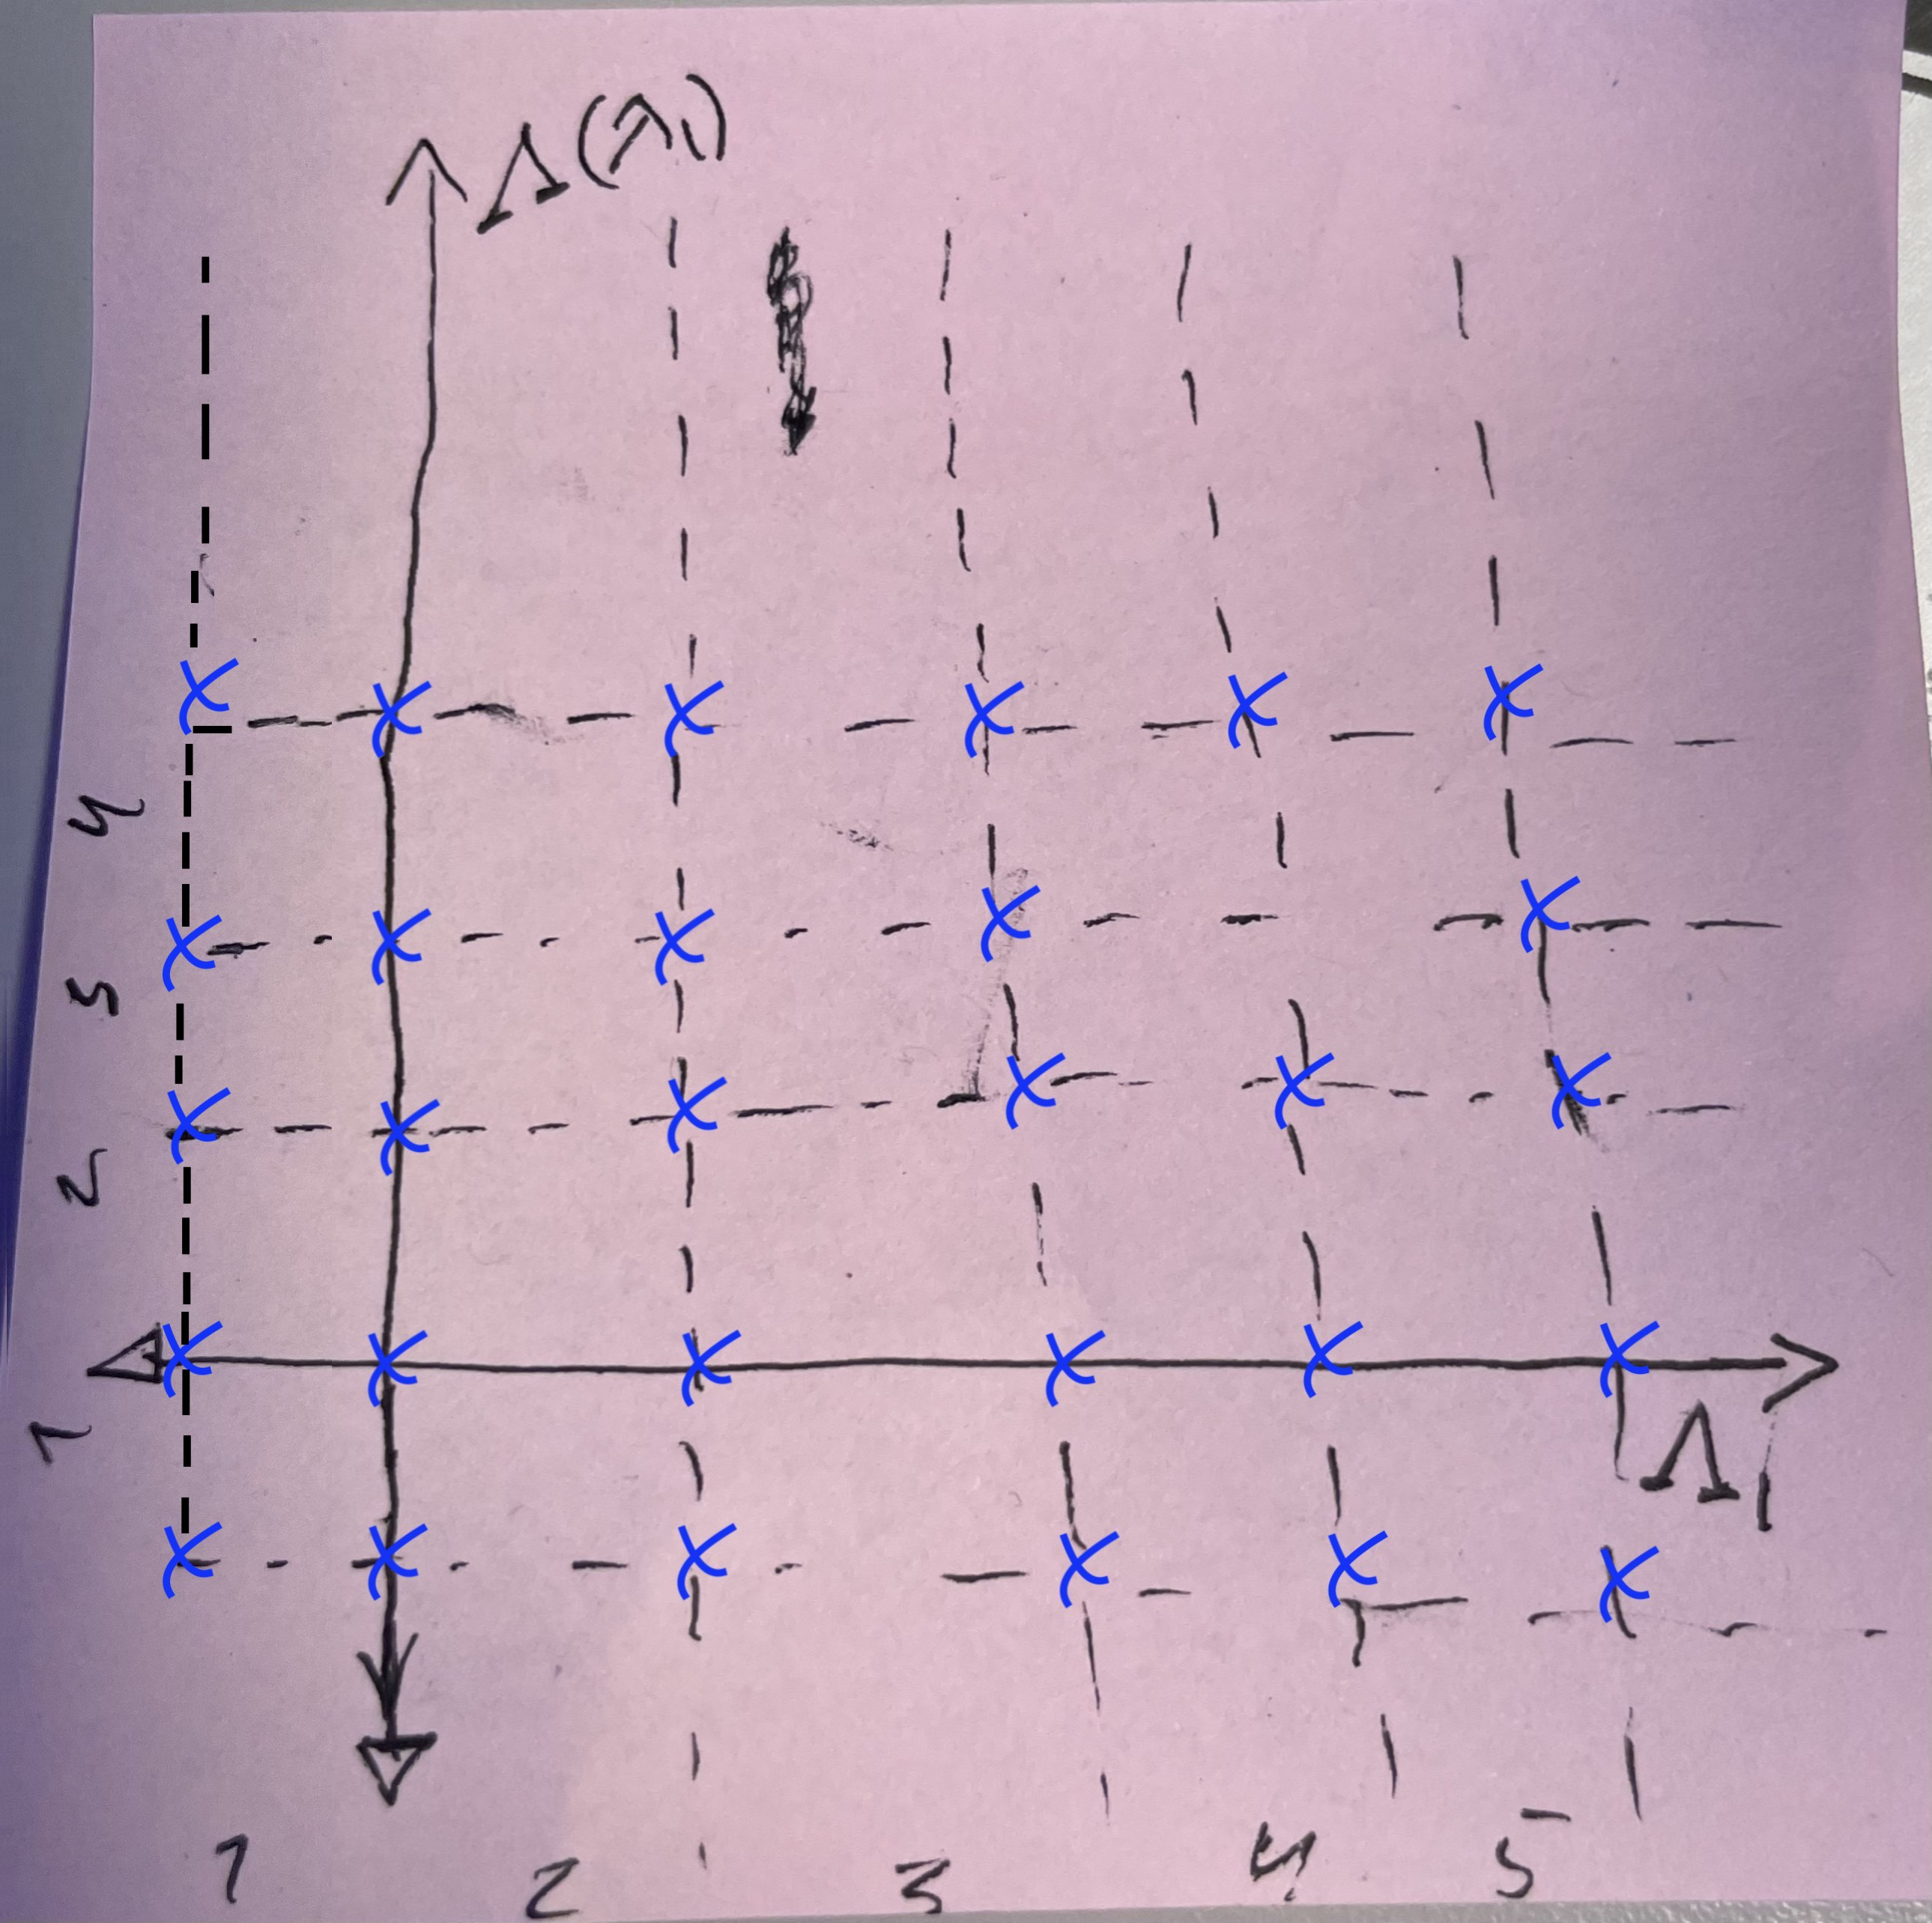
\includegraphics[width=0.9\linewidth]{spec_no_shift.jpg}
        %* Figure 1
        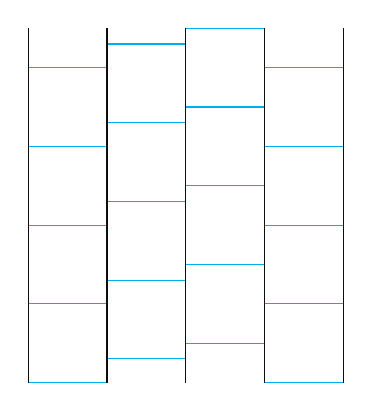
\begin{tikzpicture}[scale=1]
            % Define the tile
            \def\tile{
            %\draw (1,0) -- (1,1) -- (0,1) -- (0,0) -- cycle;  % Draw the unit square
            \draw[black!95] (0,0) rectangle (1,1);
            %\draw (0,0) rectangle (1,1);
            \draw[cyan] (0,0) -- (1,0);
            \draw[cyan] (0,1) -- (1,1);
            }
            
            % Draw the tiling pattern
            \foreach \x in {0,1,2,3}{
                \foreach \y in {0,1,2,3}{
                    % Here we shift with different z values for each height value 
                    % i.e. Row shift
                    \ifnum\x=0
                        \pgfmathsetmacro{\shiftX}{\x} % Set horizontal shift
                        \pgfmathsetmacro{\shiftY}{\y}
                    \fi
                    \ifnum\x=1
                        \pgfmathsetmacro{\shiftX}{\x} % Set horizontal shift
                        \pgfmathsetmacro{\shiftY}{\y+0.3}
                    \fi
                    \ifnum\x=2
                        \pgfmathsetmacro{\shiftX}{\x} % Set horizontal shift
                        \pgfmathsetmacro{\shiftY}{\y+0.5}
                    \fi
                    \ifnum\x=3
                        \pgfmathsetmacro{\shiftX}{\x} % Set horizontal shift
                        \pgfmathsetmacro{\shiftY}{\y}
                    \fi
                    \begin{scope}[shift={(\shiftX,\shiftY)}]
                        \tile % Draw the tile
                    \end{scope}
                }
            }
            % black lines to hide the blue lines
            \foreach \x in {0,1,2,3,4}{
                \draw[ black!95] (\x,0) -- (\x,4);
                \draw[black!95] (\x,0+0.3) -- (\x,4+0.3);
                \draw[black!95] (\x,0+0.3) -- (\x,4+0.5);
                \draw[black!95] (\x,0) -- (\x,4+0.5);
                \draw[black!95] (\x,0) -- (\x,4);
            }
        \end{tikzpicture}
        %* —————————————————
        %\caption{Lattice tiling}
        \label{fig:tiling_five}
    \end{subfigure}\quad
    \begin{subfigure}{.47\textwidth}
        \centering
        %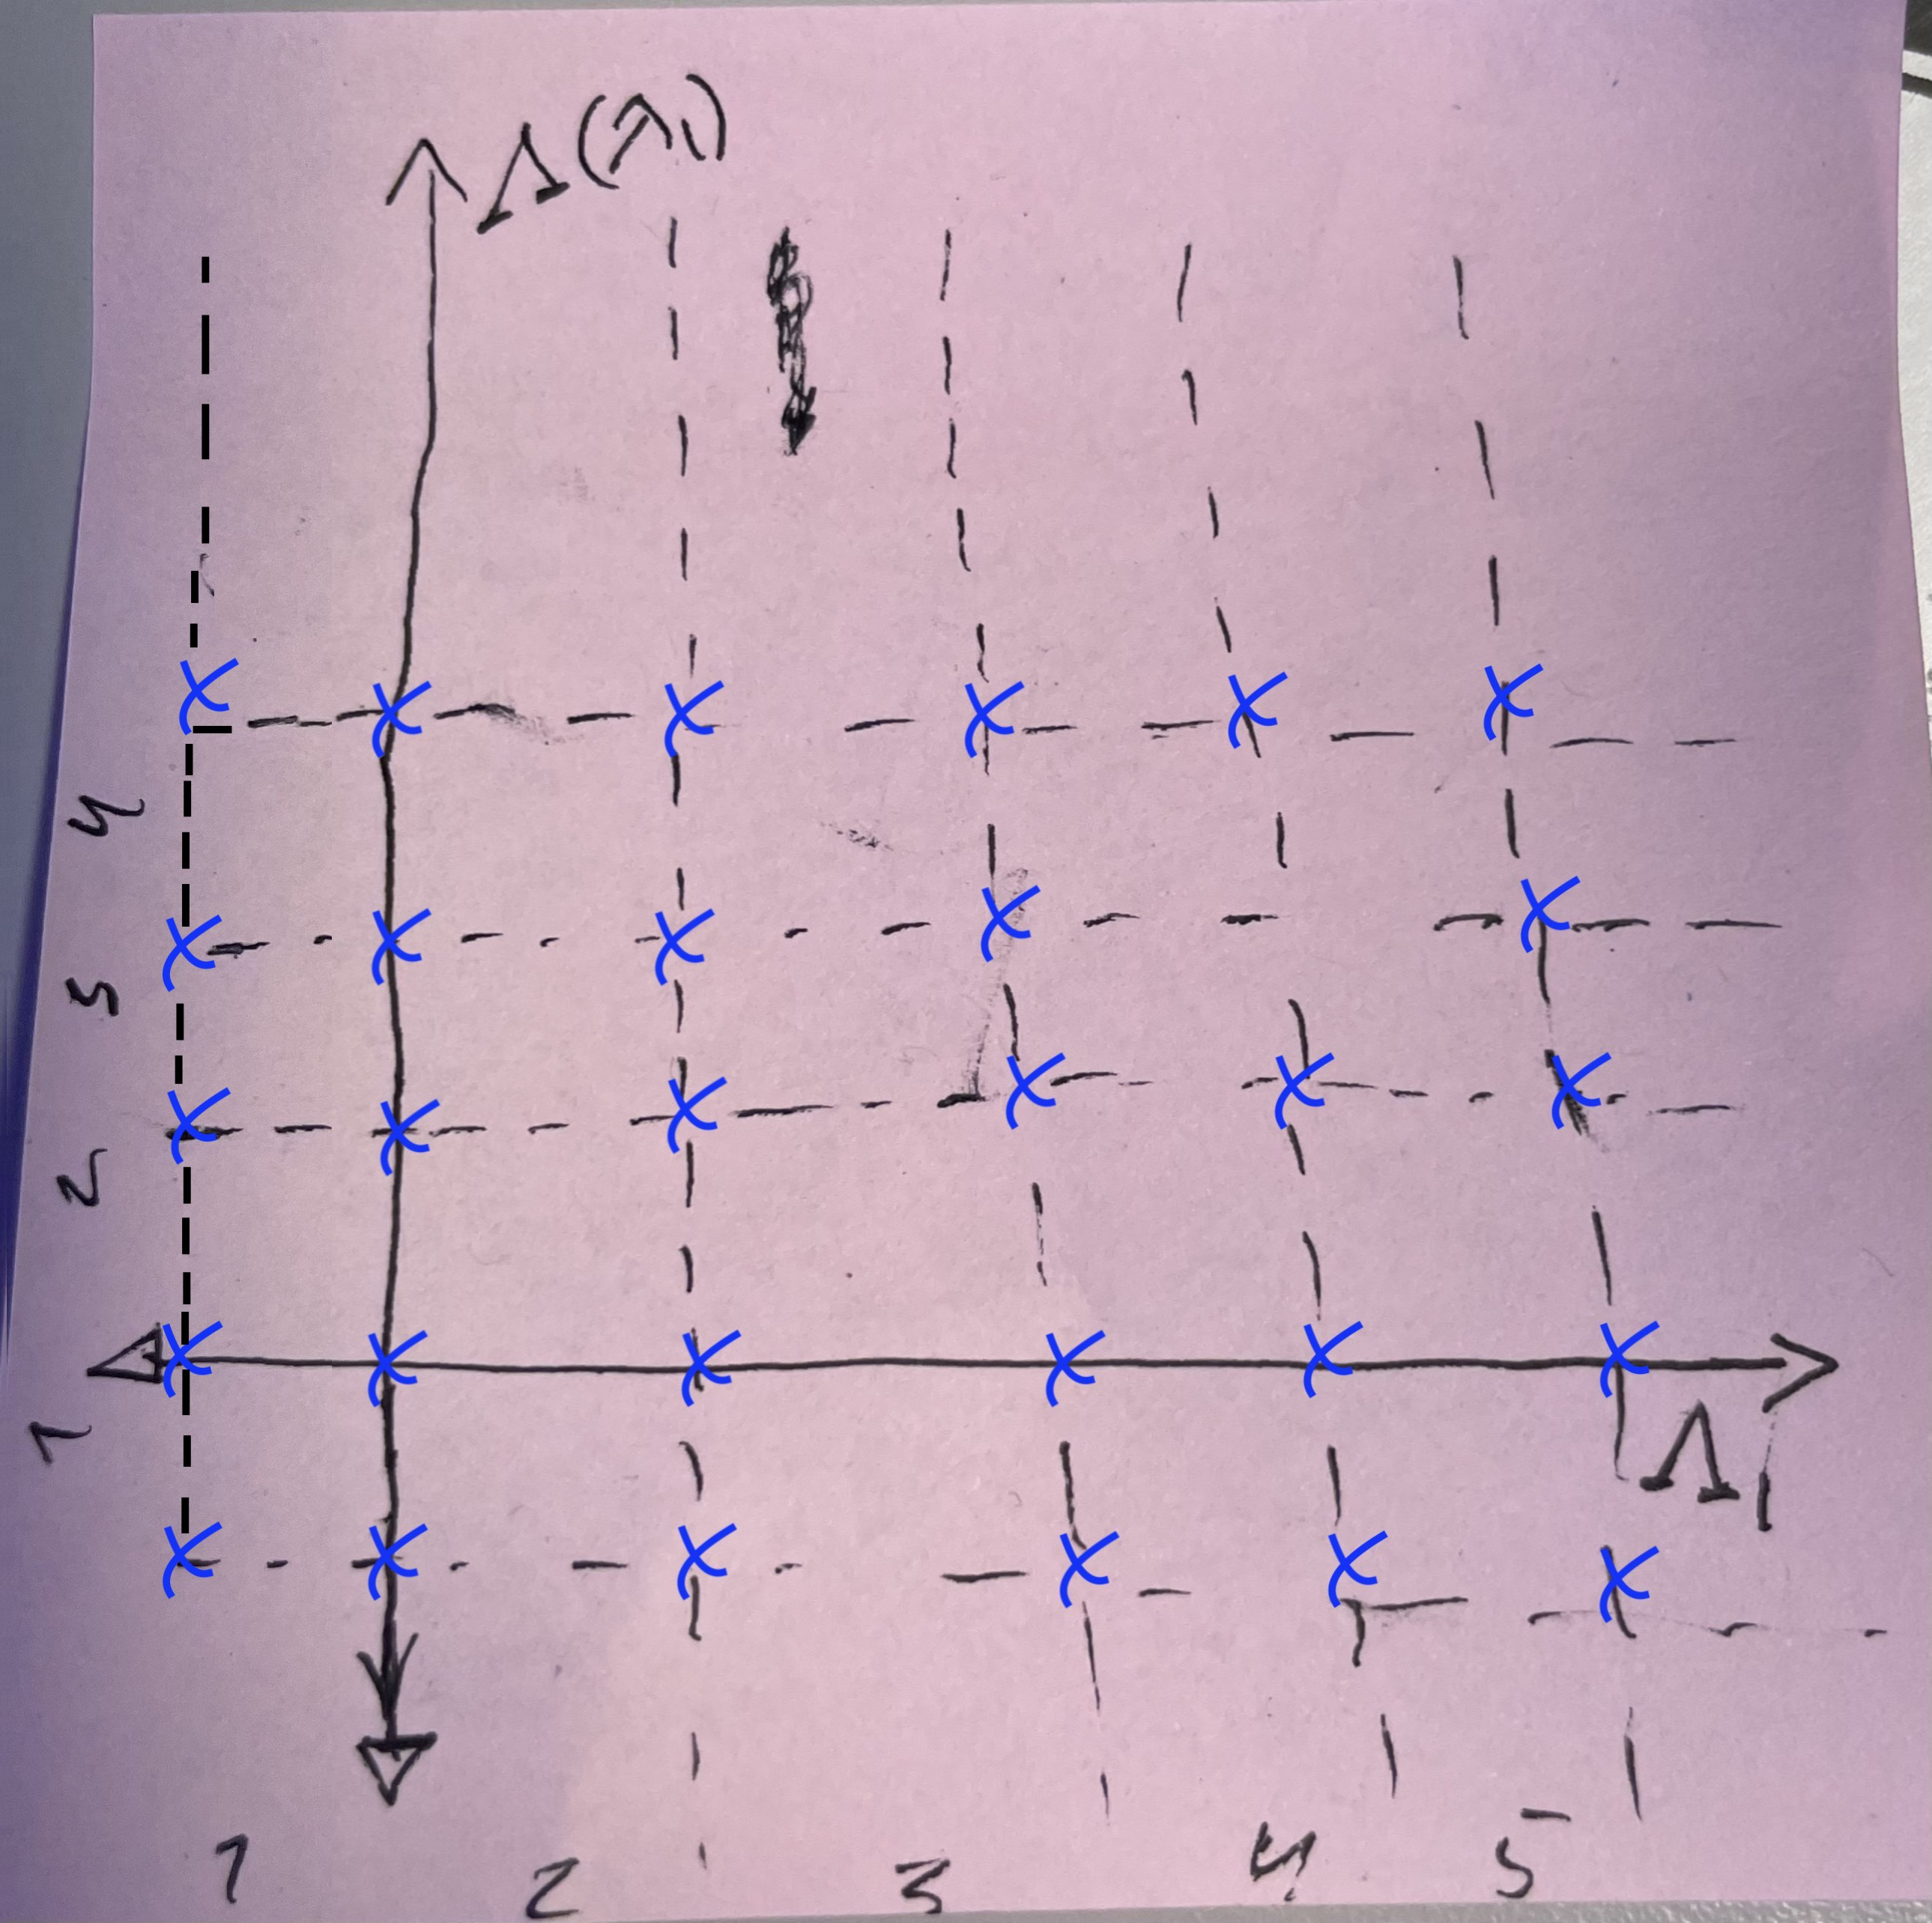
\includegraphics[width=0.9\linewidth]{spec_no_shift.jpg}
        %* Figure 1
        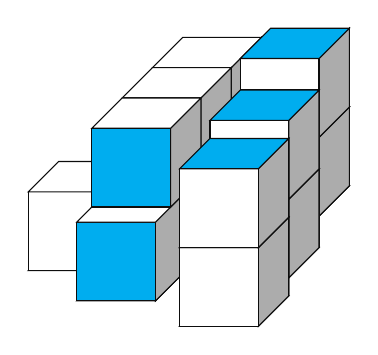
\begin{tikzpicture}[scale=1]
            % Define the tile
            \def\tile{
              % Draw the unit cube
                \draw[black!95] (1,0,0) -- (1,0,1) -- (1,1,1) -- (1,1,0) -- cycle; % left face
                \draw[black!95] (0,0,0) -- (1,0,0) -- (1,0,1) -- (0,0,1) -- cycle; % bottom face
                \draw[black!95] (0,0,0) -- (0,1,0) -- (1,1,0) -- (1,0,0) -- cycle; % back face
                \draw[black!95, fill=gray!65] (1,0,0) -- (1,1,0) -- (1,1,1) -- (1,0,1) -- cycle; % right face
                \draw[black!95, fill=white] (0,0,1) -- (1,0,1) -- (1,1,1) -- (0,1,1) -- cycle; % front face
                \draw[black!95, fill=white](0,1,0) -- (0,1,1) -- (1,1,1) -- (1,1,0) -- cycle; % top face
            }
            
            \def\tiletwo{
                % Draw the unit cube
                    \draw[black!95] (1,0,0) -- (1,0,1) -- (1,1,1) -- (1,1,0) -- cycle; % left face
                    \draw[black!95] (0,0,0) -- (1,0,0) -- (1,0,1) -- (0,0,1) -- cycle; % bottom face
                    \draw[black!95] (0,0,0) -- (0,1,0) -- (1,1,0) -- (1,0,0) -- cycle; % back face
                    \draw[black!95, fill=gray!65] (1,0,0) -- (1,1,0) -- (1,1,1) -- (1,0,1) -- cycle; % right face
                    \draw[black!95, fill=cyan] (0,0,1) -- (1,0,1) -- (1,1,1) -- (0,1,1) -- cycle; % front face
                    \draw[black!95, fill=white](0,1,0) -- (0,1,1) -- (1,1,1) -- (1,1,0) -- cycle; % top face
                }
        
            \def\tilethree{
                % Draw the unit cube
                    \draw[black!95] (1,0,0) -- (1,0,1) -- (1,1,1) -- (1,1,0) -- cycle; % left face
                    \draw[black!95] (0,0,0) -- (1,0,0) -- (1,0,1) -- (0,0,1) -- cycle; % bottom face
                    \draw[black!95] (0,0,0) -- (0,1,0) -- (1,1,0) -- (1,0,0) -- cycle; % back face
                    \draw[black!95, fill=gray!65] (1,0,0) -- (1,1,0) -- (1,1,1) -- (1,0,1) -- cycle; % right face
                    \draw[black!95, fill=white] (0,0,1) -- (1,0,1) -- (1,1,1) -- (0,1,1) -- cycle; % front face
                    \draw[black!95, fill=cyan](0,1,0) -- (0,1,1) -- (1,1,1) -- (1,1,0) -- cycle; % top face
                }
          
            % Draw the tiling pattern
            % For x=0
            \foreach \x in {0}{
               \foreach \y in {0}{
                    \foreach \z in {0}{
                        \pgfmathsetmacro{\shiftX}{\x} % Set horizontal shift
                        \pgfmathsetmacro{\shiftY}{\y} % Set vertical shift
                        \pgfmathsetmacro{\shiftZ}{\z+0.8} % Set vertical shift
                        \begin{scope}[shift={(\shiftX,\shiftY,\shiftZ)}]
                        \tile % Draw the tile
                        \end{scope}
                    }
                }
            }
            % For x=1
            \foreach \x in {1}{
               \foreach \y in {0,1}{
                    \foreach \z in {-1,0,1}{
                        % Here we shift with different z values for each height value 
                        % i.e. Row shift
                        \ifnum\y=0
                            \pgfmathsetmacro{\shiftX}{\x} % Set horizontal shift
                            \pgfmathsetmacro{\shiftY}{\y}
                            \pgfmathsetmacro{\shiftZ}{\z+0.8} % Set vertical shift
                        \fi
                        \ifnum\y=1
                            \pgfmathsetmacro{\shiftX}{\x} % Set horizontal shift
                            \pgfmathsetmacro{\shiftY}{\y}
                            \pgfmathsetmacro{\shiftZ}{\z+0.3} % Set vertical shift
                        \fi
                        \ifnum\y=2
                            \pgfmathsetmacro{\shiftX}{\x} % Set horizontal shift
                            \pgfmathsetmacro{\shiftY}{\y}
                            \pgfmathsetmacro{\shiftZ}{\z-0.5} % Set vertical shift
                        \fi
                        
                        \begin{scope}[shift={(\shiftX,\shiftY,\shiftZ)}]
                        \tiletwo % Draw the tile
                        \end{scope}
                    }
                }
            }
        
            % For x=2
            % The code for this part is a bit divided, thre last columns are here, the one in the very back has same shift as the one in the front
            \foreach \x in {2}{
               \foreach \y in {0,1}{
                    \foreach \z in {-1,0,1}{
                        % Here we shift with different y values for each depth value
                        % i.e. Column shift
                        \ifnum\z=-1
                            \pgfmathsetmacro{\shiftX}{\x} % Set horizontal shift
                            \pgfmathsetmacro{\shiftY}{\y}
                            \pgfmathsetmacro{\shiftZ}{\z} % Set vertical shift
                        \fi
                        \ifnum\z=0
                            \pgfmathsetmacro{\shiftX}{\x} % Set horizontal shift
                            \pgfmathsetmacro{\shiftY}{\y-0.4}
                            \pgfmathsetmacro{\shiftZ}{\z} % Set vertical shift
                        \fi
                        \ifnum\z=1
                            \pgfmathsetmacro{\shiftX}{\x} % Set horizontal shift
                            \pgfmathsetmacro{\shiftY}{\y-0.63}
                            \pgfmathsetmacro{\shiftZ}{\z} % Set vertical shift
                        \fi
                        \begin{scope}[shift={(\shiftX,\shiftY,\shiftZ)}]
                        \tilethree % Draw the tile
                        \end{scope}
                    }
                }
            }
        \end{tikzpicture}
        %* —————————————————
        %\caption{Lattice tiling}
        \label{fig:tiling_six}
    \end{subfigure}
    \caption{Highlighted in cyan are the fully face-sharing edges (left) and squares (right) for dimensions two and three, respectively. Observe the different orientations for the cyan squares.}
    \label{fig:tilings_five_six}
\end{figure}
